\documentclass{article}

% preamble, set properties here
\usepackage{amsmath}  % for custom math
\usepackage{graphicx} % for figures
\usepackage{parskip}  % better loooking paragraphs
\usepackage{hyperref} % for internet links
\usepackage{geometry}

% Setup margins and paper size
\geometry{
  letterpaper,
  total={170mm,257mm},
  left=20mm,
  top=20mm,
  bottom=25mm
}


\title{Rocket Altitude Trajectory Control}
\date{\today}
\author{Jeffrey Millard}

\begin{document}

%\pagenumbering{gobble}
\maketitle
%\newpage
%\pagenumbering{arabic}


\section{Introduction}
  I was approached by a member of the undergraduate AIAA club here at BYU who will be participating in a competition that involves sending a rocket to arrive precisely at 10,000 feet. With fins, the current rocket design is quite stable and we expect the rocket to climb nearly vertical. Since the rules allow anyone to contribute, I've developed a simulation environment that is available publicly on GitHub at this \href{http://www.texample.net/tikz/resources/}{link}. The simulation simulates the rocket trajectory, control, estimation, and provides structure for Monte Carlo analysis.

  While many aspects of the simulation apply to linear system theory, my final project for ECEN 773 concerns itself with the overall approach to altitude trajectory control and more specifically, the Kalman Filter design and results. The KF estimates numerous states including the drag coefficient. This allows for accurate reference trajectory updates online, which yeilds increased robustness in the face of uncertain drag parameters.

\section{The Rocket}
  The problem is framed as follows. The simulation (including estimation and control) takes place immediately following the solid propellant burn. So our system can then be thought of as having an initial altitude ($h_0$) and velocity ($\dot{h}_0$). Since the rocket is traveling vertically without wind, $\dot{h}$ is considered the same as the airspeed. The equations of motion describing the system are
  \begin{equation}
    \ddot{h} = -g -D
  \end{equation}
  where $g$ is gravity and
  \begin{equation}
    D = \frac{1}{2} \rho \dot{h}^2 \bar{CD}
  \end{equation}
  $\bar{CD}$ is simply the convention chosen to represent a given drag coefficient already multiplied by a reference area so that it doesn't need to be chosen for the current rocket. This means that $\bar{CD}$ is not unitless, but the math is equivalent so long as we are consistent. This overall drag parameter can be represented as the base drag parameter plus the increase due to the air brake angle, $\theta$, as shown here
  \begin{equation}
    \bar{CD} = \bar{CD}_0 + \frac{\delta\bar{CD}}{\delta\theta} \theta
  \end{equation}
  where $\frac{\delta\bar{CD}}{\delta\theta}$ is considered a constant parameter. Since $\rho$ depends on our states, we can express it using $h$ and other constants
  \begin{equation}
    \rho = \rho_0 \left(   \frac{T_0 - \alpha\left( h-h_0 \right)}{T_0}   \right)^{n-1}
  \end{equation}
  where $\rho_0$, $T_0$, $\alpha$, and $n$ are the initial air density, initial air temperature, atmospheric temperature change, and gas constant, respectively.

  This results in the final equation
  \begin{equation}
    \ddot{h} = -g -\frac{1}{2} \left[\rho_0 \left(   \frac{T_0 - \alpha\left( h-h_0 \right)}{T_0}   \right)^{n-1}\right] \dot{h}^2 \left(\bar{CD}_0 + \frac{\delta\bar{CD}}{\delta\theta} \theta \right)
  \end{equation}

  The airbrake dynamics are governed by
  \begin{equation}
    \ddot{\theta} = \frac{\tau}{J} - \frac{\ell}{2}D_\theta \sin \theta
  \end{equation}
  where $\tau$ is the motor torque (input), $J$ is the angular inertia, $\ell$ is the airbrake surface length, and $D_\theta \sin \theta$ is simply the added drag due to airbrake deployment tending to push the brake back to $\theta=0$. This assumes that the center of pressure for the added airbrake drag is applied to the center of the surface, hence $\frac{\ell}{2}$ used as the moment arm for resistance torque. It is also worth noting that
  \begin{equation}
    D_\theta = \frac{1}{2} \rho \dot{h}^2 \left(\frac{\delta\bar{CD}}{\delta\theta} \theta \right)
  \end{equation}
  Using the same state-dependent expression for $\rho$, the full equation for airbrake dynamics is
  \begin{equation}
    \ddot{\theta} = \frac{\tau}{J} - \frac{\ell}{4} \left[ \rho_0 \left(   \frac{T_0 - \alpha\left( h-h_0 \right)}{T_0}   \right)^{n-1} \right] \dot{h}^2 \left(\frac{\delta\bar{CD}}{\delta\theta} \theta \right) \sin \theta
  \end{equation}

  This lays the groundwork for simulation and control. In the following sections, I discuss the control and estimation approaches used.

\section{The Trajectory Approach}
  Consider a dragless object in a gravity field. Regardless of whether or not the object is falling or climbing, the map of $\dot{h}$ vs $h$ is well-defined based on gravity. Such is not the case for an object with drag. The falling and climbing trajectories of $\dot{h}$ vs $h$ will be different. The approach used here is to generate a reference trajectory of the climbing rocket using a pessimistic drag such that it reaches the desired altitude with zero remaining velocity. Since the integral cannot be easily solved in closed form while maintaining all the nonlinearities, an interative numerical approach is used to find the necessary starting velocity $h_0$ as well as the entire subsequent trajectory of $\dot{h}$ vs $h$. The idea is to control the velocity, $\dot{h}$, such that the rocket's motion converges on this trajectory without any overshoot (since we have no method of adding additional needed energy to the system). This can be done by using the reference trajectory as a look-up-table to find the desired $\dot{h}$ for any current $h$.

  The initial control approach was to use PID with successive loop closure and truth states in order to prove the concept of trajectory control. This could be improved upon using feedback linearization with the $\theta$ dynamics.

  The main problem to be addressed by this project is the observability and estimation of the base drag coefficient. In order to grasp the motivation, consider the case where little is known about the drag of the system. One might simply put large variance on the drag coefficient during Monte Carlo simulation, but eventually the question arrises: how pessimistic does the drag need to be for the generation of the reference trajectory? If it isn't pessimistic enough such that the real drag is greater than expected, then controlling the the reference trajectory means the rocket will inevitably slow down past the trajectory, undershooting the target altitude. If it is too pessimistic, then we have a situation where too much control is needed at the tail end of the flight when there perhaps isn't enough time to shed the excess energy, resulting in overshooting the target altitude.

  To address this problem, I created an Extended Kalman Filter that estimates relevant states as well as the base drag parameter, $\bar{CD}_0$. This allows for an online update of the reference trajectory to avoid the problems described above.

\section{The States and Linearization}
  One possible state configuration is
  \begin{equation}
    x = \left[\begin{matrix} h \\
                             \dot{h} \\
                             \theta \\
                             \dot{\theta} \\
                             \bar{CD}_0         \end{matrix}\right]
      = \left[\begin{matrix} x_1 \\
                             x_2 \\
                             x_3 \\
                             x_4 \\
                             x_5         \end{matrix}\right]
  \end{equation}

  By inspection of equations 5 and 8, we see that the only possible equilibrium point requires $\dot{h}$ to be zero which eliminates all of our nonlinearities which would make some states unobservable. For an initial first step, we use the Jacobian linearization about the current operating point. It is true that the current operating point cannot be made an equilibrium point regardless of the input. One workaround would be to use the Indirect Kalman Filter in order to use error states which doesn't have the same problem with equilibrium points. Since this construction is used only for the observer, I use the Jacobian linearization about the operating point. While this is expected to introduce some error, I tuned Q to minimize it and I show later that this produces good results. Another thing I did was to augment the state vector with gravity. This is done so that the linearization of $\ddot{h}$ doesn't completely neglect the acceleration from gravity in order to get better state estimate propagation. The resulting state vector is
  \begin{equation}
    x = \left[\begin{matrix} h \\
                             \dot{h} \\
                             \theta \\
                             \dot{\theta} \\
                             \bar{CD}_0 \\
                             g          \end{matrix}\right]
      = \left[\begin{matrix} x_1 \\
                             x_2 \\
                             x_3 \\
                             x_4 \\
                             x_5 \\
                             x_6        \end{matrix}\right]
  \end{equation}
  and full nonlinear state dynamics in terms of states and constants:
  \begin{equation}
    \dot{x} = f(x,u) = \left[\begin{matrix} x_2 \\
                                            -x_6 -\frac{1}{2} \left[\rho_0 \left(   \frac{T_0 - \alpha\left( x_1-h_0 \right)}{T_0}   \right)^{n-1}\right] x_2^2 \left(x_5 + \frac{\delta\bar{CD}}{\delta\theta} x_3 \right) \\
                                            x_4 \\
                                            \frac{u}{J} - \frac{\ell}{4} \left[ \rho_0 \left(   \frac{T_0 - \alpha\left( x_1-h_0 \right)}{T_0}   \right)^{n-1} \right] x_2^2 \left(\frac{\delta\bar{CD}}{\delta\theta} x_3 \right) \sin x_3 \\
                                            0 \\
                                            0        \end{matrix}\right]
  \end{equation}

  With the Jacobian, the standard linearized form yields
  \begin{equation}
    \dot{x} = Ax + Bu
  \end{equation}
  where
  \begin{equation}
    A = \left[\begin{matrix} 0 & 1 & 0 & 0 & 0 & 0                   \\
                             \frac{\delta \dot{x_2}}{\delta x_1} & \frac{\delta \dot{x_2}}{\delta x_2} & \frac{\delta \dot{x_2}}{\delta x_3} & 0 & \frac{\delta \dot{x_2}}{\delta x_5} & -1                      \\
                             0 & 0 & 0 & 1 & 0 & 0                    \\
                             \frac{\delta \dot{x_4}}{\delta x_1} & \frac{\delta \dot{x_4}}{\delta x_2} & \frac{\delta \dot{x_4}}{\delta x_3} & 0 & 0 & 0                      \\
                             0 & 0 & 0 & 0 & 0 & 0                      \\
                             0 & 0 & 0 & 0 & 0 & 0              \end{matrix}\right]
  \end{equation}
  \begin{equation}
    B = \left[\begin{matrix} 0 \\
                             0 \\
                             0 \\
                             J^{-1} \\
                             0 \\
                             0      \end{matrix}\right]
  \end{equation}
  and partial derivatives are
  \begin{equation}
    \frac{\delta \dot{x_2}}{\delta x_1} = \frac{\rho_0 \alpha}{2 T_0}x_2^2 \left( x_5 + \frac{\delta \bar{CD}}{\delta \theta} x_3 \right) \left( n-1 \right) \left( \frac{T_0-\alpha \left( x_1 - h_0\right)}{T_0} \right)^{n-2}
  \end{equation}
  \begin{equation}
    \frac{\delta \dot{x_2}}{\delta x_2} = -\rho_0 \left( \frac{T_0-\alpha \left( x_1 - h_0\right)}{T_0} \right)^{n-1} x_2 \left( x_5 + \frac{\delta \bar{CD}}{\delta \theta} x_3 \right)
  \end{equation}
  \begin{equation}
    \frac{\delta \dot{x_2}}{\delta x_3} = -\frac{1}{2}\rho_0 \left( \frac{T_0-\alpha \left( x_1 - h_0\right)}{T_0} \right)^{n-1} x_2^2 \frac{\delta \bar{CD}}{\delta \theta}
  \end{equation}
  \begin{equation}
    \frac{\delta \dot{x_2}}{\delta x_5} = -\frac{1}{2}\rho_0 \left( \frac{T_0-\alpha \left( x_1 - h_0\right)}{T_0} \right)^{n-1} x_2^2
  \end{equation}
  and
  \begin{equation}
    \frac{\delta \dot{x_4}}{\delta x_1} = \frac{\rho_0 \alpha \ell}{4 T_0}x_2^2 \frac{\delta \bar{CD}}{\delta \theta} x_3 \left(n-1 \right) \left( \frac{T_0-\alpha \left( x_1 - h_0\right)}{T_0} \right)^{n-2} \sin x_3
  \end{equation}
  \begin{equation}
    \frac{\delta \dot{x_4}}{\delta x_2} = -\frac{\rho_0 \ell}{2}\left( \frac{T_0-\alpha \left( x_1 - h_0\right)}{T_0} \right)^{n-1} x_2 \frac{\delta \bar{CD}}{\delta \theta} x_3 \sin x_3
  \end{equation}
  \begin{equation}
    \frac{\delta \dot{x_4}}{\delta x_3} = -\frac{\rho_0 \ell}{2}\left( \frac{T_0-\alpha \left( x_1 - h_0\right)}{T_0} \right)^{n-1} x_2^2 \frac{\delta \bar{CD}}{\delta \theta} x_3
  \end{equation}

  Updating these partial derivatives at each iteration allows the creation of an EKF.

  \section{Observability}

  A proper observability analysis would consider the full nonlinear state dynamics using Lie derivatives to generate the observability matrix. This could be considered out of the scope of the class. Further, one can intuitively conclude that the drag parameter is only observable when $\rho$ and $\dot{h}$ are both nonzero. Nevertheless, we can do a basic observability analysis using the $A$ matrix presented above.

  Using barometer and angle encoders, we have direct measurement of $h$ and $\theta$($x_1$ and $x_3$). Since gravity is known and constant, we have a pseudo measurement for it without noise. Therefore our measurement model is reflected by
  \begin{equation}
    C = \left[\begin{matrix} 1 & 0 & 0 & 0 & 0 & 0  \\
                             0 & 0 & 1 & 0 & 0 & 0  \\
                             0 & 0 & 0 & 0 & 0 & 1              \end{matrix}\right]
  \end{equation}
  Using this, we can generate an observability matrix in general form (not assuming values for the partial derivatives).
  \begin{equation}
    \mathcal O = \left[\begin{matrix} C  \\
                                      CA  \\
                                      CA^2 \\
                                      \vdots \\
                                      CA^{n-1}            \end{matrix}\right]
               = \left[\begin{matrix} 1 & 0 & 0 & 0 & 0 & 0  \\
                                      0 & 0 & 1 & 0 & 0 & 0  \\
                                      0 & 0 & 0 & 0 & 0 & 1  \\
                                      0 & 1 & 0 & 0 & 0 & 0  \\
                                      0 & 0 & 0 & 1 & 0 & 0  \\
                                      0 & 0 & 0 & 0 & 0 & 0  \\
                                      \frac{\delta \dot{x_2}}{\delta x_1}& \frac{\delta \dot{x_2}}{\delta x_2}& \frac{\delta \dot{x_2}}{\delta x_3}& 0& \frac{\delta \dot{x_2}}{\delta x_5}& -1 \\
                                      \frac{\delta \dot{x_4}}{\delta x_1}& \frac{\delta \dot{x_4}}{\delta x_2}& \frac{\delta \dot{x_4}}{\delta x_3}& 0&   0&  0 \\
                                      0  &   0&   0& 0&   0&  0 \end{matrix}\right]
  \end{equation}
  We see that this remains full rank so long as $\frac{\delta \dot{x_2}}{\delta x_5}$ ($\frac{\delta \ddot{h}}{\delta \bar{CD}_0}$) remains nonzero. This is the equivalent of saying that we can only detect the drag parameter so long as the rocket's acceleration is still affected by it. This is something to keep in mind as the rocket nears the end of simulation. Extra logic may be required to hold the converged constant drag parameter value once $\dot{h}$ drops below a chosen threshold.




  \section{Results}
  Figure 1 shows the overall result of the rocket under closed-loop control. It is seen that the the current truth trajectory gradually approaches the reference trajectory. In this realization, the error drops a bit negative (dropping below the reference trajectory), but the final altitude of 3043.4m (9985ft) was satisfactory. It can be noted that with some additional attention, the control performance could be improved with feedback linearization.

  \begin{figure}
    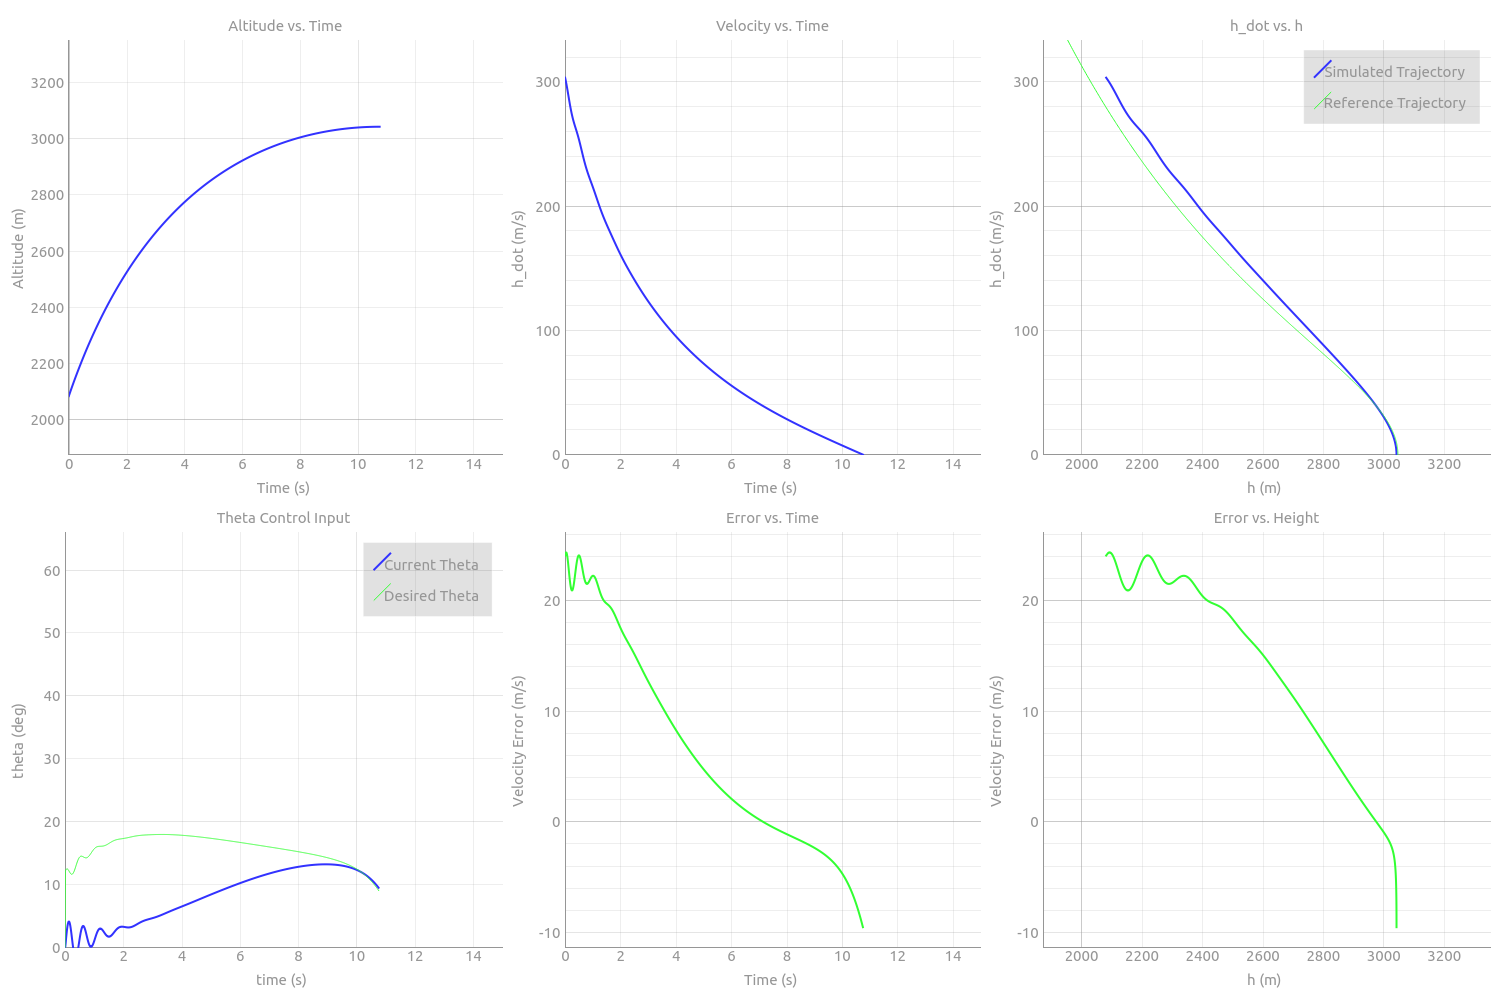
\includegraphics[width=\linewidth]{figures/main.png}
    \caption{The rocket simulation showing the states of interest.}
    \label{fig:main}
  \end{figure}

  More importantly, Figure 2 shows the the estimated and 

  \begin{figure}
    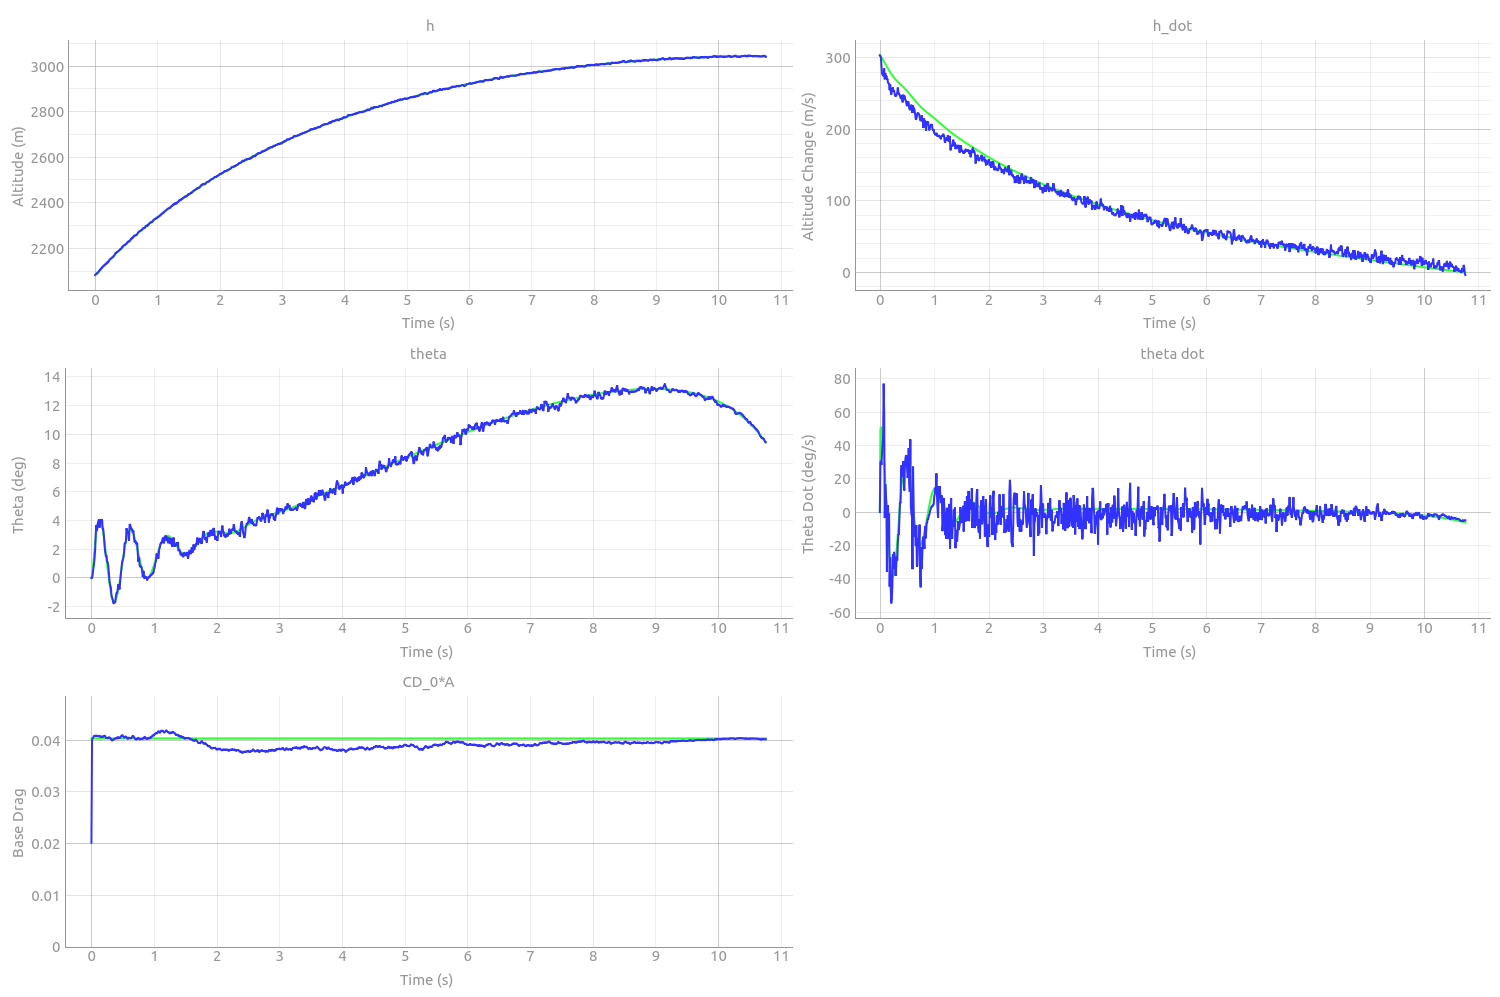
\includegraphics[width=\linewidth]{figures/estimates.png}
    \caption{The state estimates versus truth. Green represents truth and Blue represents the estimate}
    \label{fig:estimates}
  \end{figure}

  % explain drag parameter more explicitly so that the reference area might be chosen later
  % then compared to other rockets easier

  % explain better that the sim obeyed full nonlinear models

\end{document}
